\newpage
\subsection{Design}

Formålet med dette kapitel er at planlægge løsningen, ud fra de krav der der er
stillet, sammenholdt med erfaringerne fra analysen.

%Skal indeholde Overvejelser, beslutninger og resultater vedr.
%Softwarearkitektur og detaljeret design, herunder design af persistens. 

\subsubsection{Trelagsarkitektur}%
\label{ssub:3_lags_arkiteturen}
%i denne sektion beskrives vores tre-lags arkitektur.
%Lokalisering af ændringer

Kravet om en trelagsarkitektur (IF-01) er markeret om et "must" i prioriteringen af
krav. I FURPS+ analysen er kravet placeret som en "Design constraint", da dette
stiller et krav til designet af systemets arkitektur. 

%Hvordan kan lagene separeres? 

\paragraph{Interfaces} Et oplagt værktøj til at opdele lagene i
trelagsarkitekturen er anvendelse af interfaces. Med interfaces i mellem lagene 
skal hver enkelt lag kun afhænge af det specificerede interface. På denne måde
er der indgået en \emph{kontrakt} i mellem de to pågældende lag.
Ved anvendelse af disse interfaces behøves det lag der anvender interfacet ikke
at kende til selve implementationen af interfacet.

\paragraph{Separation mellem præsentationslaget og domænelaget}

Et designmønster der er en oplagt som en del af trelagsarkitekturen er
designmønsteret 'Model-View-Controller'\cite[p. 176]{} . Dette designmønster er struktureret
således:

\renewcommand{\baselinestretch}{1}
\begin{figure}[H]
    \centering
    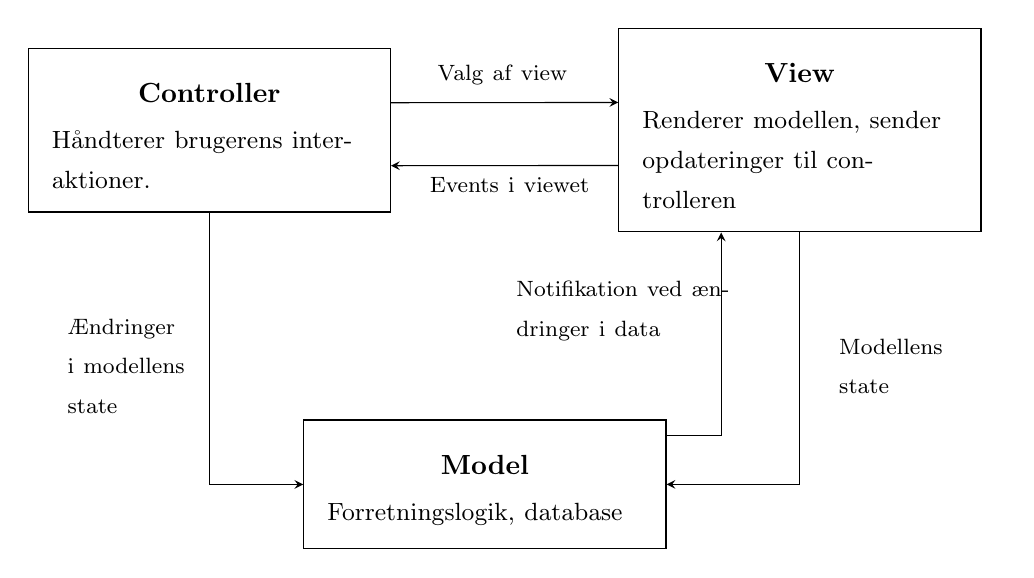
\begin{tikzpicture}
        \node[rectangle, draw, text width=4cm, inner sep=3mm] (view) at (7.5,0) 
            { \vspace{-4mm}\begin{center}
                    \textbf{View}
                \end{center}
            %\hline
            \vspace{-2mm} \small
             Renderer modellen, sender opdateringer til controlleren};
        \node[rectangle, draw, text width=4cm, inner sep=3mm] (controller) at
            (0,0) 
            { \vspace{-4mm}\begin{center}
                    \textbf{Controller}
                \end{center}
            %\hline
            \vspace{-2mm} \small
            Håndterer brugerens interaktioner.};
        \node[rectangle, draw, text width=4cm, inner sep=3mm] (model) at
            (3.5,-4.5) 
            { \vspace{-4mm}\begin{center}
                    \textbf{Model}
                \end{center} \small
            %\hline
            \vspace{-2mm}
            Forretningslogik, database};
        \node[text width=3cm] (nodetoview ) at (4.4, 0.7) {\footnotesize{Valg af view}};
        \node[text width=3cm] (tocontroller) at (4.3, -0.7) {\footnotesize{Events i viewet}};
        \node[text width=3cm] (nodetoview ) at (5.4, -2.3) {\footnotesize{Notifikation ved ændringer i data}};
        \node[text width=2cm] (modeltoview ) at (9, -3) {\footnotesize{Modellens state}};
        \node[text width=2cm] (controllertomodel ) at (-0.8, -3) {\footnotesize{Ændringer i modellens state}};
        \draw[-stealth] ([yshift= -0.7cm]controller.north east) -- ([yshift= -0.95cm]view.north west);
        \draw[stealth-] ([yshift= -1.5cm]controller.north east) -- ([yshift= -1.75cm]view.north west);
        \draw[-stealth] ([yshift= -0.2cm]model.north east) -| ([xshift= -1cm]view.south);
        \draw[stealth-] (model.east) -| (view.south);
        \draw[-stealth] (controller.south) |- (model.west);
    \end{tikzpicture} 
    \label{fig:mvc}
\end{figure}
\renewcommand{\baselinestretch}{1.2}

Dette designmønster separerer interaktion og præsentation fra systemets data.
Det vil sige at præsentations- og domænelaget separeres. View \emph{observerer}
data der holdes i modellen. View præsenterer det data der holdes i modellen til
brugeren. Dette gør at data kan ændre sig uafhængigt af præsentationen, siden
præsentationslaget udelukkende observerer data.  Controlleren står for at
respondere på der sker i view, fx hvis en bruger klikker på et element der skal
starte et nyt view, da står den for det sætte det nye view til at blive vist.
Den står også for at håndtere hvad der gøres når der klikkes på et given element
i viewet.  Modellen repræsenterer de to andre lag, forretningslogiklaget og
persistenslaget, og står derved for håndtere og manipulere med data.

\paragraph{Separation mellem domænelaget og persistenslaget}

For at separere domænelaget persistenslaget, man der anvendes andet
designmønster. Generelt set kan man sige at domænelaget anvender
persistenslaget. For at simplificere kommunikationen mellem domænelaget og
persistenslaget kan vi anvende én klasse til at interagere med persistenslaget.
Dette designmønster kaldes "Facade"-designmønsteret. Denne facadeklasse skjuler
den konkrete implementation af persistenslaget.

For at specificere en egentlig kontrakt, som persistenslaget skal leve op til
kan der specificeres et interface, for de operationer som persistenslaget skal
tilbyde.

\paragraph{Abstraktion af dataobjekter}

Selv om systemets opdeles i tre lag, skal data stadig kunne flyde i mellem de
tre lag. Her er det vigtigt at de samme dataobjekter anvendes i alle lag. For at
sikre at et lag (fx præsentationslaget) kan anvende af et dataobjekt skal der
specificeres en kontrakt der stille krav for implementationen af hvert
dataobjekt. Præsentationslaget kan derfor nu afhænge af interfacet(kontrakten)
og de metoder denne tilbyder, i stedet for at afhænge direkte på
implementationen af et givent dataobjekt. Dermed kan implementationen af det
underliggende dataobjekt ændre sig, selvom det tilbyder de samme operationer (da
det stadig skal leve op til kontrakten).

\subsubsection{Subsystemer}%
\label{ssub:subsystemer}

Dekomposition er en vigtig del af at dekonstruerere et større system ned i flere
små dele. På denne måde bliver vores system mere håndtérbart. Subsystemer
separeres med interfaces, således at de deles fra resten af systemet. Disse
interfaces sørger for at der er en pålidelig kontaktflade med resten af
programmet.

I analyse klassediagrammet på figur \ref{fig:AnalyseKlasseDiagramV3} er klassen overdrevet komplekt. Der er svær at se sig ud af og har alt for mange ansvarsområder. Denne klasse kunne deles op i flere klasser der hver knytter siger til at arbejde (manage) en type af kreditering. Derved står ApplicationManager for at have styr på klasserne, og de yderligere klasser (managers) står for at have styr på de specifikke typer af krediteringer/dataobjekter. 

Som det ses i pakkediagrammet på figur \ref{fig:PackageDiagram} 
eksisterer der en \texttt{services} pakke. Denne pakke tilbyder services for
hvert type af dataobjekt. Dette betyder at data for hvert dataobjekt er
separeret fra \texttt{ApplicationManager}, således at GUI kan observere data fra
præcis den nødvendige liste, og ikke har adgang til andre lister med data i
klassen. På denne måde undgås en enkelt gudeklasse, der har adgang til al data,
og de operationer der tilbydes på den givne data.

\begin{figure}[H]
    \centering
    \begin{tikzpicture}
        \begin{umlpackage}{presentation}
            \begin{umlpackage}{GUI}
            \end{umlpackage}{GUI}
        \end{umlpackage}
        \begin{umlpackage}{domain}
            \begin{umlpackage}[x=6]{services}
            \end{umlpackage}
        \end{umlpackage}
    \umlassemblyconnector[interface=MovieManager, anchors=east and west]{GUI}{services}
    \end{tikzpicture}
    \caption{Interface mellem service og præsentationslaget}
\end{figure}

Yderligere valgte gruppen et design, der frakobler instantieringen af objekter fra DatabaseLoaderen, ved at lave en pakke/system der hedder objectMapping. Når en burger vælger at søge fra GUI kaldes en funktion search i applicationManager. Applicationmanager vil så sørge for at der bliver søgt på alle typer af objekter. Det vil sige den først f.eks. vil kalde PersonManager som vil søge efter krediteringer af typen Person. I første iteration blev disse person objekter instantieret direkte på DatabaseLoaderen. Men da objektKlasserne lå i domænelaget overholdte dette ikke  tre-lags-modllen, og samtidig ville det også skabe problemer, hvis vi i fremtiden ville tilføje flere variabler til et objekt da dette er tæt koblet. I stedet valgte gruppen at afkolbe denne instantiering af objekter. Det bringer os tilbage til objectMapping. Designet blev sådan, at når der søges, returnerer DatabaseLoader blot et ResultSet fra databasen, og så står objectMapping så for at iterere over dette ResultSet og instantiere objekter derfra. Derved ville man blot skulle ændre én klasse inde i objectMapping for at sørge for, nye variabler bliver medtaget.


\subsubsection{Pakkediagram} Systemet er delt op i pakker efter præsentations-,
domæne- og persistenslag. Ved denne opdeling kan det nemmere sikres at
trelagsarkitekturen overholdes. Et pakkediagram blev opsat og kan ses på figur
\ref{fig:PackageDiagram}

\begin{figure}[H]
    \centering
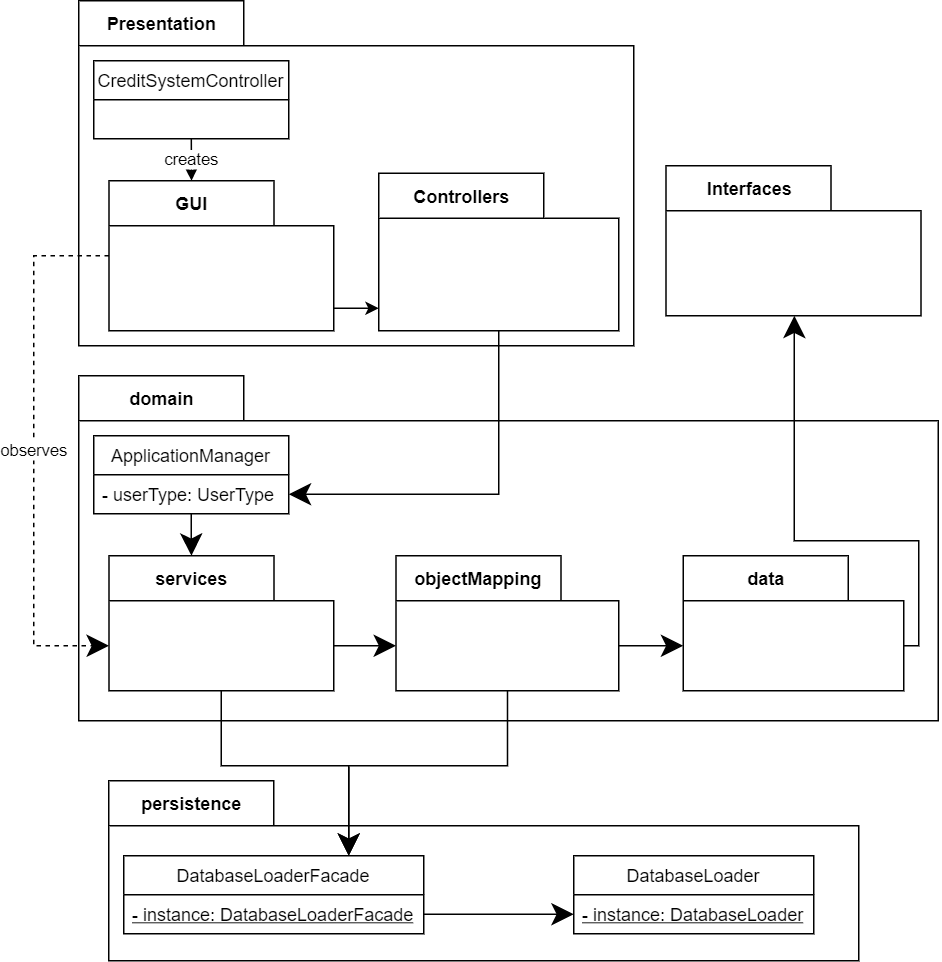
\includegraphics[scale = 0.3]{images/PackageDiagram.png}
    \caption{Pakkediagram for systemet}
    \label{fig:PackageDiagram}
\end{figure}

Figur \ref{fig:PackageDiagram} viser hvordan pakkerne kommunikerer med hinanden.
Klassen CreditSystemController, viser en GUI for brugeren. Når brugeren
foretager en handling, knytter GUI sig til nogle controllers i pakken
Controllers som kalder metoder på ApplicationManager i domænelaget.
ApplicationManager kalder den passende Manager i pakken Services som kan gøre en
af to ting: 

\begin{itemize}
    \item Hvis brugeren har oprettet en ny kreditering i GUI er objektet
        allerede instantieret, og manageren kalder derfor en 'put' metode på
        DatabaseLoaderFacade i persistenslaget, som derefter kalder den passende
        metode i Databaseloader. 
    \item Hvis brugeren har søgt efter en kreditering, kalder manageren først
        pakken object Mapping, som herefter kalder en 'get' funktion på
        Databaseloadeefacade som dernæst kalder den passende metode på
        Databaseloader der querier databasen, og returnerer resultaterne. Disse
        resultater får object Mapping pakken, og indstanierer objekter via data
        pakken i domain.
\end{itemize}

Gruppen valgte at lave en facade til DatabaseLoader, hvor al kommunikation med DatabaseLoader skal ske igennem. DatabaseLoaderFacade har bl.a. flere overloadede metoder ved navn putInDatabse som tager forskellige typer af objekter, alt efter hvad brugeren vælger at tilføje. Dette gør det nemt at lave funktioner der skal skrive til databasen, da der ikke er 10 forskellige funktioner man skal huske navnene på, men blot kan kalde 'put' metoden med en type af objekt, og så kalder facaden selv den rigtige metode i DatabaseLoader






\subsubsection{Klassediagram}%
\label{ssub:klassediagram}


\subsubsection{Systemsekvensdiagrammer}%
\label{ssub:systemsekvensdiagrammer}
Ved brug af dette design, dannede gruppen et meget detaljeret sekvensdiagram over B03: Foretage en søgning, for at visualisere flowet i programmet som kan ses på figur \ref{fig:B03OSDDesign}

\begin{figure}
    %\centering
    \makebox[\textwidth][c]{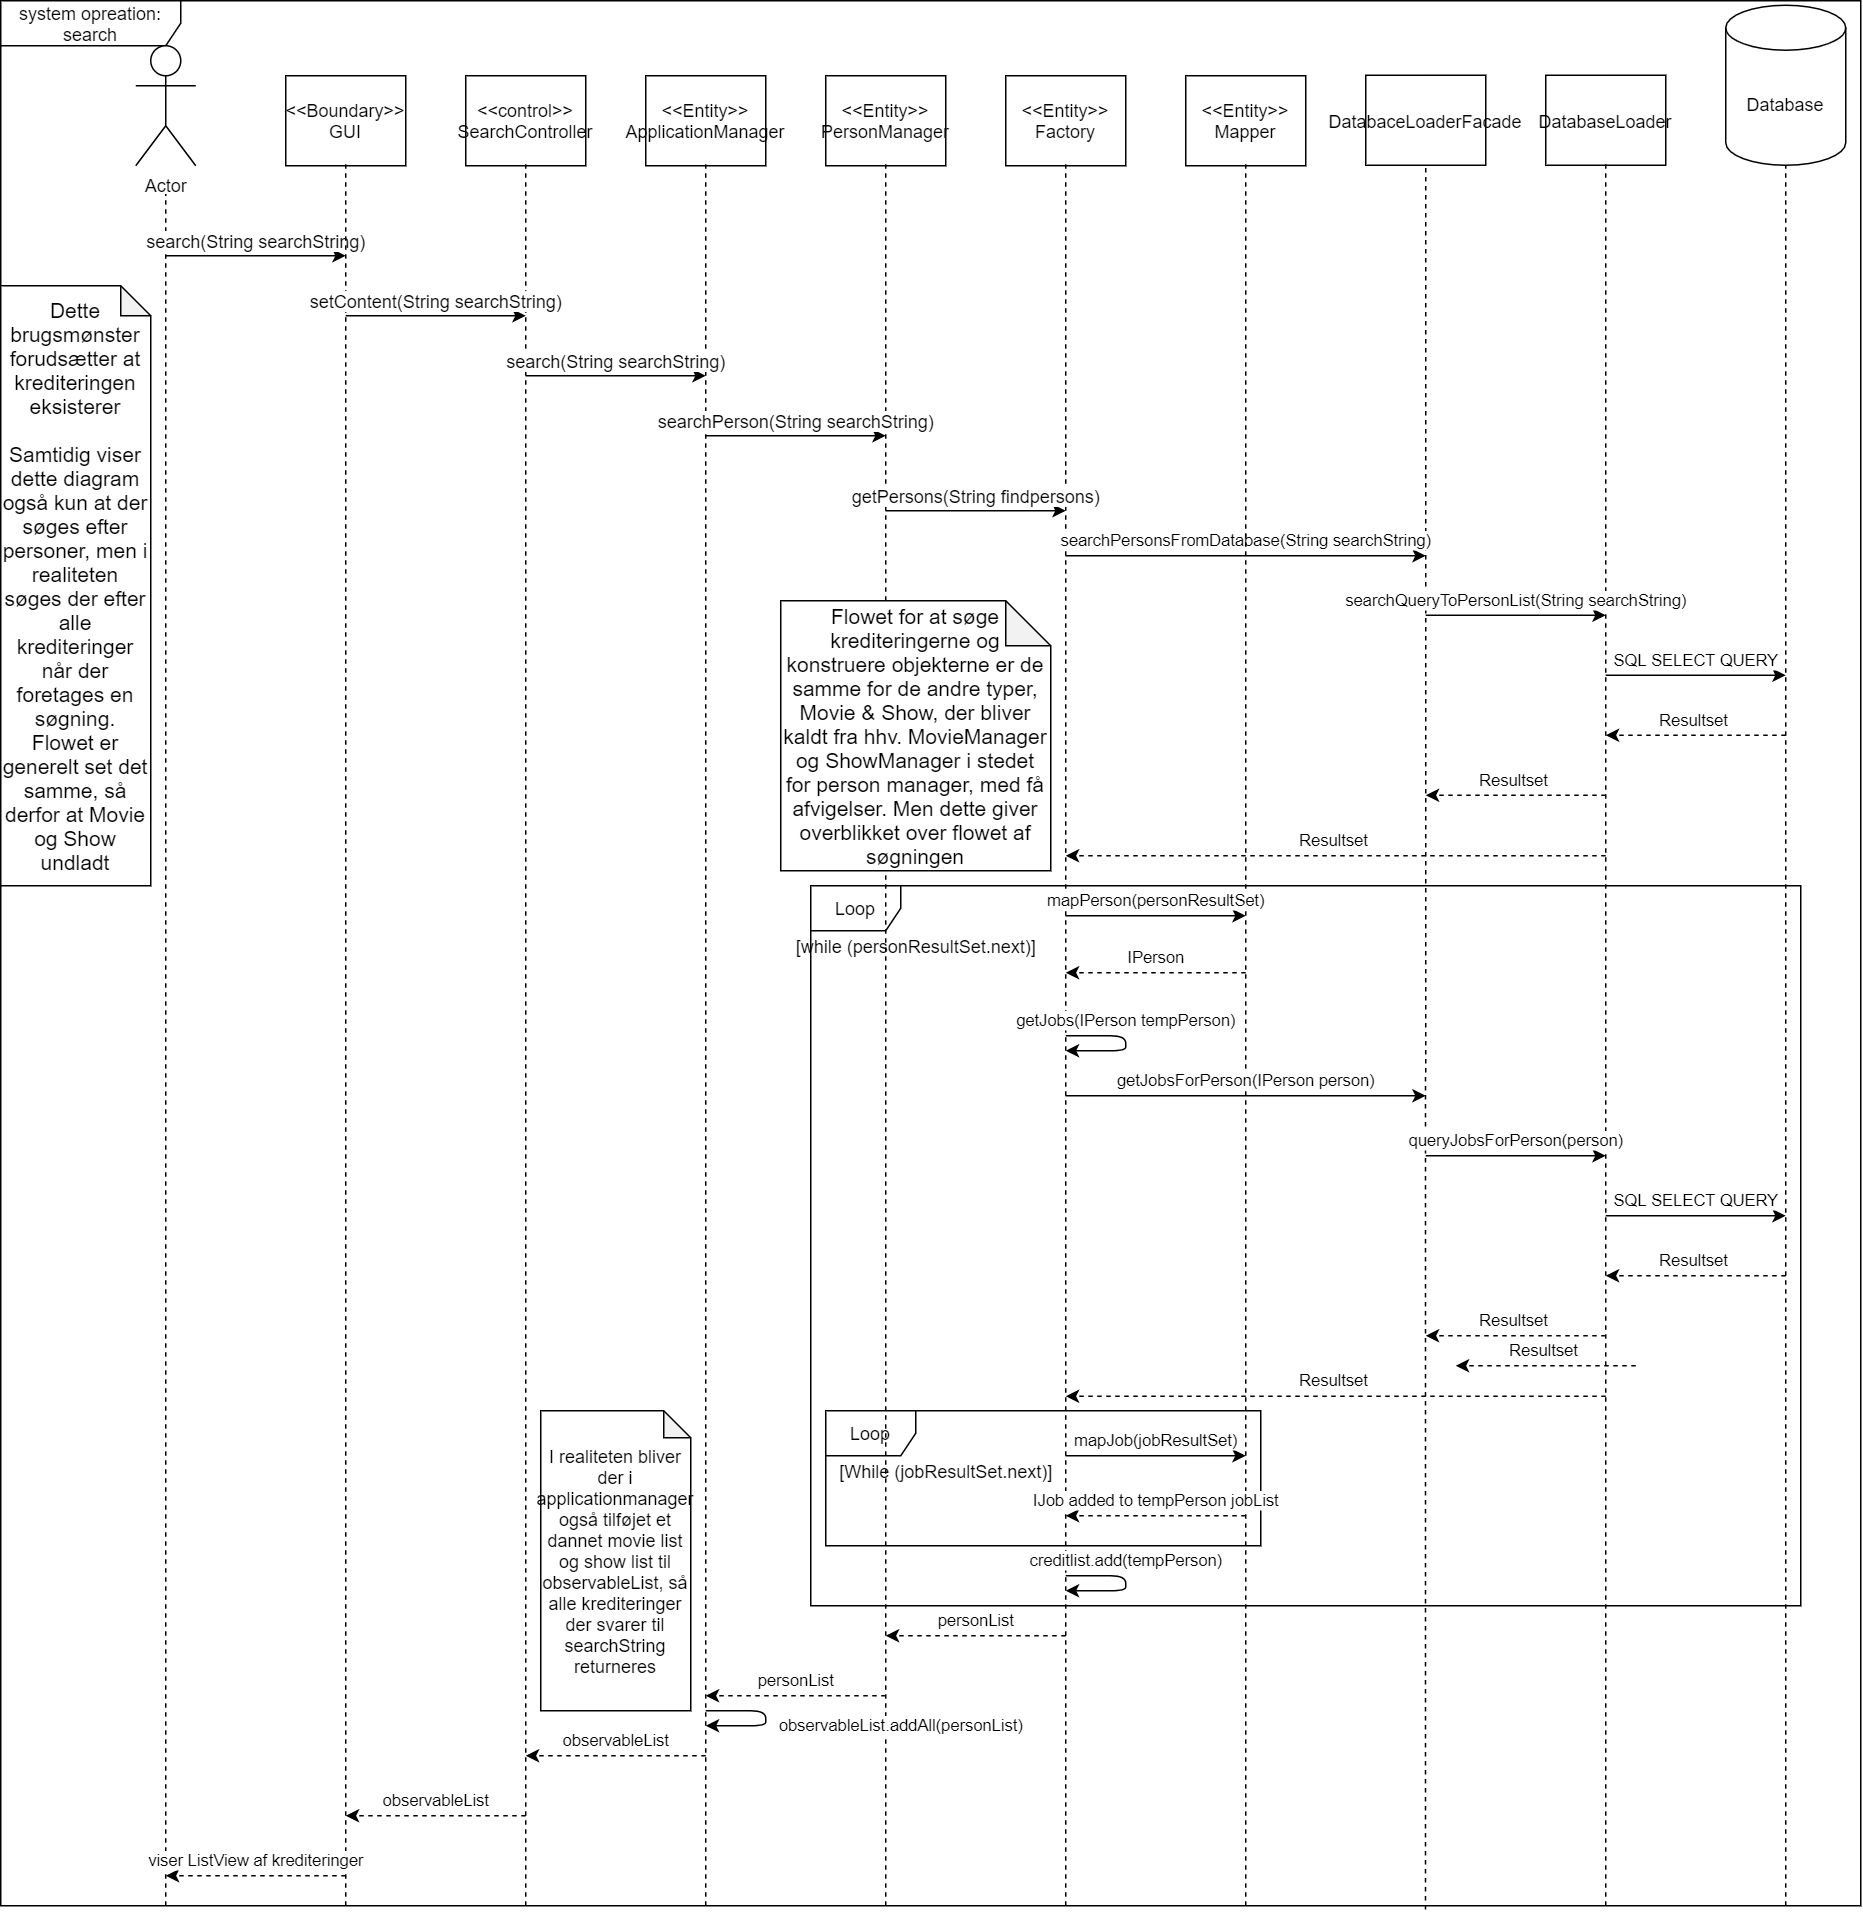
\includegraphics[width=1.25\textwidth]{images/B03OSDDesign.png}}
    \caption{Design sekvensdiagram for search funktionaliteten}
    \label{fig:B03OSDDesign}
\end{figure}

Operations sekvensdiagrammet på figur \ref{fig:B03OSDDesign} viser hvilke klasser som systemet går igennem for at lave en søgning. Det starter med at aktøren indtaster sine søgekriterier og trykker søg på GUI'en. Dette kalder funktionen search som tager en string som parameter. Search kalder funktionen setContent på SearchController klassen, som har til ansvar at få en liste fra searchString og vise den liste på GUI. SearchController kalder så funktionen search på application manager, som tager searchString og søger efter de forskellige typer af krediteringer. I dette eksempel vises kun søgningen efter personer, men flowet er det samme for film og serier, og derfor er de ikke medtaget i diagrammet. Application manager kalder searchPerson på PersonManager. PersonManager står for mange af funktonerne på objekter af typen Person. Personmanager kalder derefter getPersons på Factory. Factory er den klasse der står for at afgøre objekter der skal konstrueres og hvor data skal hentes fra. Factory kalder så searchPersonsFromDatabase på DatabaseLoaderFacade og sender igen searchString videre. DatabaseLoaderFacade er den simple indgang til databseLoader, hvor Facaden kalder funktionen searchQueryToPersonList stadig med searchString som parameter. Denne funktion queryer så databasen ved at finde de tupler der minder som søgekriteriet searchString. Databasen returnerer derefter et ResultSet af tupler, som sendes tilbage til Factory gennem DatabaseLoader, og DatabaseLoaderFacade. Her begynder konstruktionen af objekterne. Factory starter et loop, der slutter når der ikke er flere tupler i ResultSettet. For hver tupel, kalder Factory mapPerson på Mapper og sender en tupel som parameter. Metoden mapPersons tager denne tupel, og instantierer et person-objekt som en IPerson. En produktion som denne person har været med på kaldes et job. Factory sender den nyligt instantierede person til databasen (ved samme flow som perons) og får returneret et ResultSet af Jobs der har personens personID. Factory starter igen et loop over alle tupler i ResultSettet og tilføjer et instantieret job til en Arrayliste som sættes til personens jobs variabel. Her er personen konstrueret færdig, og personen tilføjes til et liste af krediteringer, creditList. og loopet kører igen. Når der ikke er flere tupler, returneres creditList, først gennem PersonManager, til ApplicationManger der tilføjer listen med personer til en generel list af Krediteringer. Her vil ApplicationManager så søge efter de nadre typer af krediteringer, film og serier, og tilføje dem til listen også. Når dette er gjort, laves listen om til en ObservableList som returneres til SearchController som sætter et ListView på GUI til at vise denne Observable list, og her får aktøren så vist listen af krediteringer der svarer til deres søgning.